\cxset{style37/.style={
 name=CHAPTER,
 numbering=Roman,
 number font-size=small,
 number font-family = rmfamily,
 number font-weight= bold,
 number before=\kern0.5em,
 number position=rightname,
 chapter font-family= sffamily,
 chapter font-weight= bold,
 chapter font-size=small,
 chapter spaceout=soul,
 number after=\par,
 chapter before=,
 chapter after=,
 chapter color=black!90,
 number color=black!90,
 title margin top=10pt,
 title margin bottom=33pt,
 title border-width=0pt,
 title padding=0pt,
 title before=,
 title after=,
 title font-family= rmfamily,
 title font-color= black!80,
 title font-weight= sfseries,
 title font-size=huge,
 chapter title align=none,
 chapter title text-align=left,
 title display=block,
 chapter title width=\textwidth,
 chapter afterindent=false}%
 }

\cxset{style37}

\chapter[Template 37]{Introduction to Style Thirty Seven}

The interesting part of this style is that it uses roman numerals to display the counter that is in a different font than that used for the chapter name.
\medskip

\begin{figure}[ht]
\centering
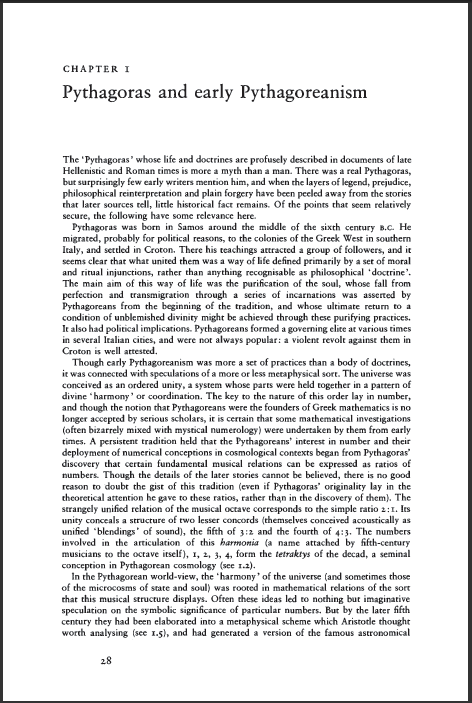
\includegraphics[width=0.6\textwidth]{./chapters/chapter37.png}
\end{figure}

\section{Running heads}

The running heads are a bit out of the ordinary as they are not displayed flushed with the margins. 
